%%%%%%%%%%%%%%%%%%%%%%%%%%%%%%%%%%%%%%%%%
% University/School Laboratory Report
% LaTeX Template
% Version 3.1 (25/3/14)
%
% This template has been downloaded from:
% http://www.LaTeXTemplates.com
%
% Original author:
% Linux and Unix Users Group at Virginia Tech Wiki 
% (https://vtluug.org/wiki/Example_LaTeX_chem_lab_report)
%
% License:
% CC BY-NC-SA 3.0 (http://creativecommons.org/licenses/by-nc-sa/3.0/)
%
%%%%%%%%%%%%%%%%%%%%%%%%%%%%%%%%%%%%%%%%%

%----------------------------------------------------------------------------------------
%	PACKAGES AND DOCUMENT CONFIGURATIONS
%----------------------------------------------------------------------------------------

\documentclass{article}

\usepackage[version=3]{mhchem} % Package for chemical equation typesetting
\usepackage{siunitx} % Provides the \SI{}{} and \si{} command for typesetting SI units
\usepackage{graphicx} % Required for the inclusion of images
\usepackage{natbib} % Required to change bibliography style to APA
\usepackage{amsmath} % Required for some math elements 
\usepackage{enumerate} % Required for the enumerate function
\usepackage[americanvoltages,siunitx]{circuitikz} % Required for the drawing of circuit diagrams
\usepackage{caption}
\usepackage{graphicx}
\usepackage{subcaption}
\usepackage{xfrac}
\usepackage{float}
\usepackage{enumitem}

\setlength\parindent{0pt} % Removes all indentation from paragraphs

\renewcommand{\labelenumi}{\alph{enumi}.} % Make numbering in the enumerate environment by letter rather than number (e.g. section 6)

%\usepackage{times} % Uncomment to use the Times New Roman font

%----------------------------------------------------------------------------------------
%	DOCUMENT INFORMATION
%----------------------------------------------------------------------------------------

\title{Electrical Circuit Analysis \\ Practical 1 - Use of function generators and digital oscilloscopes \\ ENG223} % Title

\author{Shane \textsc{Reynolds}} % Author name

\date{\today} % Date for the report

\begin{document}

\maketitle % Insert the title, author and date

\begin{center}
\begin{tabular}{l r}
Date Performed: & September 7, 2015 \\ % Date the experiment was performed
Instructor: & Dr Kamal Debnath % Instructor/supervisor
\end{tabular}
\end{center}

% If you wish to include an abstract, uncomment the lines below
% \begin{abstract}
% Abstract text
% \end{abstract}

%----------------------------------------------------------------------------------------
%	SECTION 1
%----------------------------------------------------------------------------------------

\section{Objective}

To establish an understanding of how to use a function generator to generate sinusoidal ac voltages, and to use a digital oscilloscope to measure voltages of different frequencies. Further, the practical seeks to develop understanding of how to measure phase difference between two waveforms of the same frequency.

\subsection{Background}
\label{definitions}
\begin{description}
\item[Measuring the voltage gain]
Voltage gain, in decibels, is measured using the following formula: 

\begin{align}
G = 20 \log (\frac{V_{out}}{V_{in}}) \si{\decibel}
\end{align}

where

\begin{description}[labelindent=1cm]
\item $G = \text{voltage gain}$
\item $V_{in} = \text{input voltage}$
\item $V_{out} = \text{output voltage}$
\end{description}

\newpage

\item[Measuring the phase shift]
Consider two sinusoidal voltage waveforms with some peak voltage $V_m$:

\begin{align*}
	V_{in} &= V_m \cos(\omega t - \phi_{in}) \\
	V_{out} &= V_m \cos(\omega t - \phi_{out})
\end{align*}

The phase shift between the two waveforms is measured by $|\phi_{in} - \phi_{out}|$. On the digital oscilloscope we can only measure the difference between the two nearest peaks on the waveforms, $|\Delta X|$. This is a measurement in time. To obtain a measurement in radians, we multiply by the angular frequency, that is:

\begin{align*}
	|\phi_{in} - \phi_{out}| = 2 \pi f |\Delta X| \si{\radian}
\end{align*}

The $f$ above is of course frequency in $\si{\hertz}$. Finally to get our phase shift in degrees, we multiply by the conversion factor:

\begin{align*}
	|\phi_{in} - \phi_{out}| = 2 \pi f |\Delta X| \frac{360}{2 \pi} \si{\degree}
\end{align*}

Finally, we get the following expression for calculating the phase shift in degrees from readings on our oscilloscope:

\begin{align}
	|\phi_{in} - \phi_{out}| = 360|\Delta X|f  \si{\degree}
\end{align}

where

\begin{description}[labelindent=1cm]
	\item $|\phi_{in} - \phi_{out}| = \text{phase shift}$
	\item $|\Delta X| = \text{smallest time difference between voltage peaks}$
	\item $f = \text{frequncy in \si{\hertz}}$
\end{description}

\end{description} 

\newpage

%----------------------------------------------------------------------------------------
%	SECTION 2
%----------------------------------------------------------------------------------------

\section{Experimental Circuit Set-up, Results and Calculations}

To conduct this instrumentation familiarisation practical, a simple series RC circuit was set up as shown in figure 1. The input voltage, $V_{in}$, was a sinusoidal voltage source generated by the function generator. The output voltage, $V_{out}$, was measured across the capacitor.

%Circuit Diagram
\begin{figure}[H]
\centering
\ctikzset {bipoles/length=.8cm}
\begin{circuitikz}[scale=0.6]
		
		\draw (0,0)
		to [sV, l=$V_{in}$] (0,4)
		to [R, l=$R$] (4,4)
		to [C, v^<=$C$] (4,0)
		to [short] (0,0)
		;
		
\end{circuitikz}
\captionof{figure}{Series RC circuit with Sinusoidal Input Voltage}
\label{fig:figure2}
\end{figure}

%Results table for frequency 1kHz
The frequency of the sinusoidal input voltage was set to 1 $\si{\kilo \hertz}$, 100 $\si{\kilo \hertz}$ and 1 $\si{\mega \hertz}$. The input voltage ($V_{in}$), output voltage ($V_{out}$) and the time difference ($|\Delta X|$) were recorded for each of the three frequencies. Using the recorded results, the gain was calculated using equation (1) and the phase shift, in degrees, was calculated using equation (2). Both results and calculation can be seen in table 1.
 
\begin{figure}[H]
\centering
\begin{tabular}{ | r | r | r | r | r | r | }
	\hline
	$f$ & $V_{in}$ & $V_{out}$ & $|\Delta X|$ & Gain $\si{\decibel}$ & Phase Shift $\si{\degree}$ \\ \hline
	1 \si{\hertz} & 5.108 \si{\volt} & 5.108 \si{\volt} & 0 \si{\second} & 0.00$\si{\decibel}$ & 0$\si{\degree}$ \\ \hline
	1 \si{\kilo\hertz} & 5.143 \si{\volt} & 3.353 \si{\volt} & 160 \si{\micro\second} & -3.71$\si{\decibel}$ & 57.6$\si{\degree}$ \\ \hline
	100 \si{\kilo\hertz} & 5.123 \si{\volt} & 45.15 \si{\milli\volt} & 2.462 \si{\micro\second} & -41.09$\si{\decibel}$ & 88.63$\si{\degree}$ \\ \hline
	1 \si{\mega\hertz} & 5.147 \si{\volt} & 4.480 \si{\milli\volt} & 2.650 \si{\nano\second} & -61.20$\si{\decibel}$ & 0.954$\si{\degree}$ \\ \hline 
	
\end{tabular}
\captionof{table}{Output characteristic}
\end{figure}

The results in table 1 were captured using a digital oscilloscope. To measure the magnitude of the voltage in and the voltage out, one of the trace lines on the digital oscilloscope was set on the peak and the other on the trough of the output or input sinusoidal curve. This is shown in figure 2 for the input voltage with a 1kHz frequency. To measure the phase difference, the time delay from peak to peak of the input voltage and output voltage was measured using the trace lines on the oscilloscope. This is show in figure 3 where measurements were taken for the 100kHz frequency signal.

\begin{figure}[H]
	\begin{minipage}{.6\textwidth}
		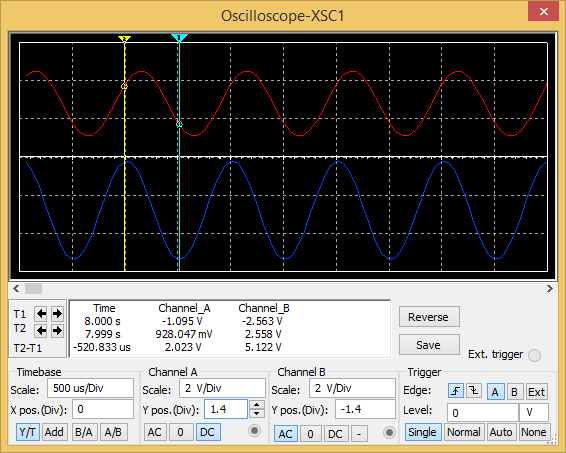
\includegraphics[scale=.4]{1kHz_inputvoltage}
		\captionof{figure}{Plot of 1kHz input signal vs.\\
			output signal. The input signal is signal \\
			B on the bottom, and the output signal \\
			is signal A on the top.}
	\end{minipage}
	\begin{minipage}{.6\textwidth}
		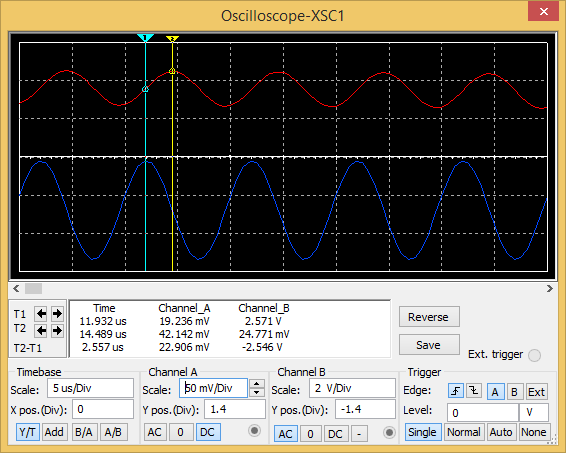
\includegraphics[scale=.4]{100kHz_time}
		\captionof{figure}{Plot of 100kHz input signal vs.\\
			output signal. The input signal is signal \\
			B on the bottom, and the output signal \\
			is signal A on the top.}
	\end{minipage}
\end{figure}

%----------------------------------------------------------------------------------------
%	SECTION 3
%----------------------------------------------------------------------------------------

\section{Problems Encountered}


The principal problem that was encountered was that the results that were recorded during the actual practical were incorrect. This was evident due to the fact that as the frequency of the circuit was increased from 1kHz to 1MHz, the output signal should have attenuated. The output voltage taken over the capacitor sees the circuit act as a low pass filter. The empirical data, however, did not show attenuation at higher level frequencies. To resolve this issue the circuit was simulated using National Instruments MultiSim. The results presented in the table were taken from this simulation and are in line with expectations.

The primary problem that was encountered when using the simulation software was the inability to accurately place the peak to peak voltage for the input voltage at 5V - something that was easy to do with laboratory set up. It must be noted, hwoever, that this practical is not results critical as it was simply aiming to familiarise students with the technical set up of equipment, develop techniques for result measurement, and demonstrate routine calculation of circuit gain and phase shift.

%----------------------------------------------------------------------------------------
%	SECTION 3
%----------------------------------------------------------------------------------------

\section{Conclusion}
The digital oscilloscope can be used to measure the magnitude of both input and output signals. Further, it can be used to measure the phase shift between input and output signals. Calculation of the phase shift requires a conversion from radians in order to get a degree measurement.
\end{document}